\documentclass[english,openright ,hidelinks,pdftex, 12 pt,a4, class=article,crop=false]{standalone}
\usepackage[utf8]{luainputenc}
\usepackage{geometry}
\geometry{verbose, inner=1cm, outer=1cm, bmargin=1cm, tmargin=1cm}

\setlength{\parindent}{0bp}
\usepackage{import}
\usepackage[subpreambles=false]{standalone}
\usepackage{amsmath}
\usepackage{amssymb}
\usepackage{esint}
\usepackage{babel}
\makeatletter
\makeatother
\usepackage{babel}
\usepackage{graphicx}
\usepackage{float}
\usepackage{subfig}
\usepackage{comment}
\begin{document}
\thispagestyle{empty}
Kan du finne eit rektangel med sammer verdi for omkrets og areal?
\begin{center}
	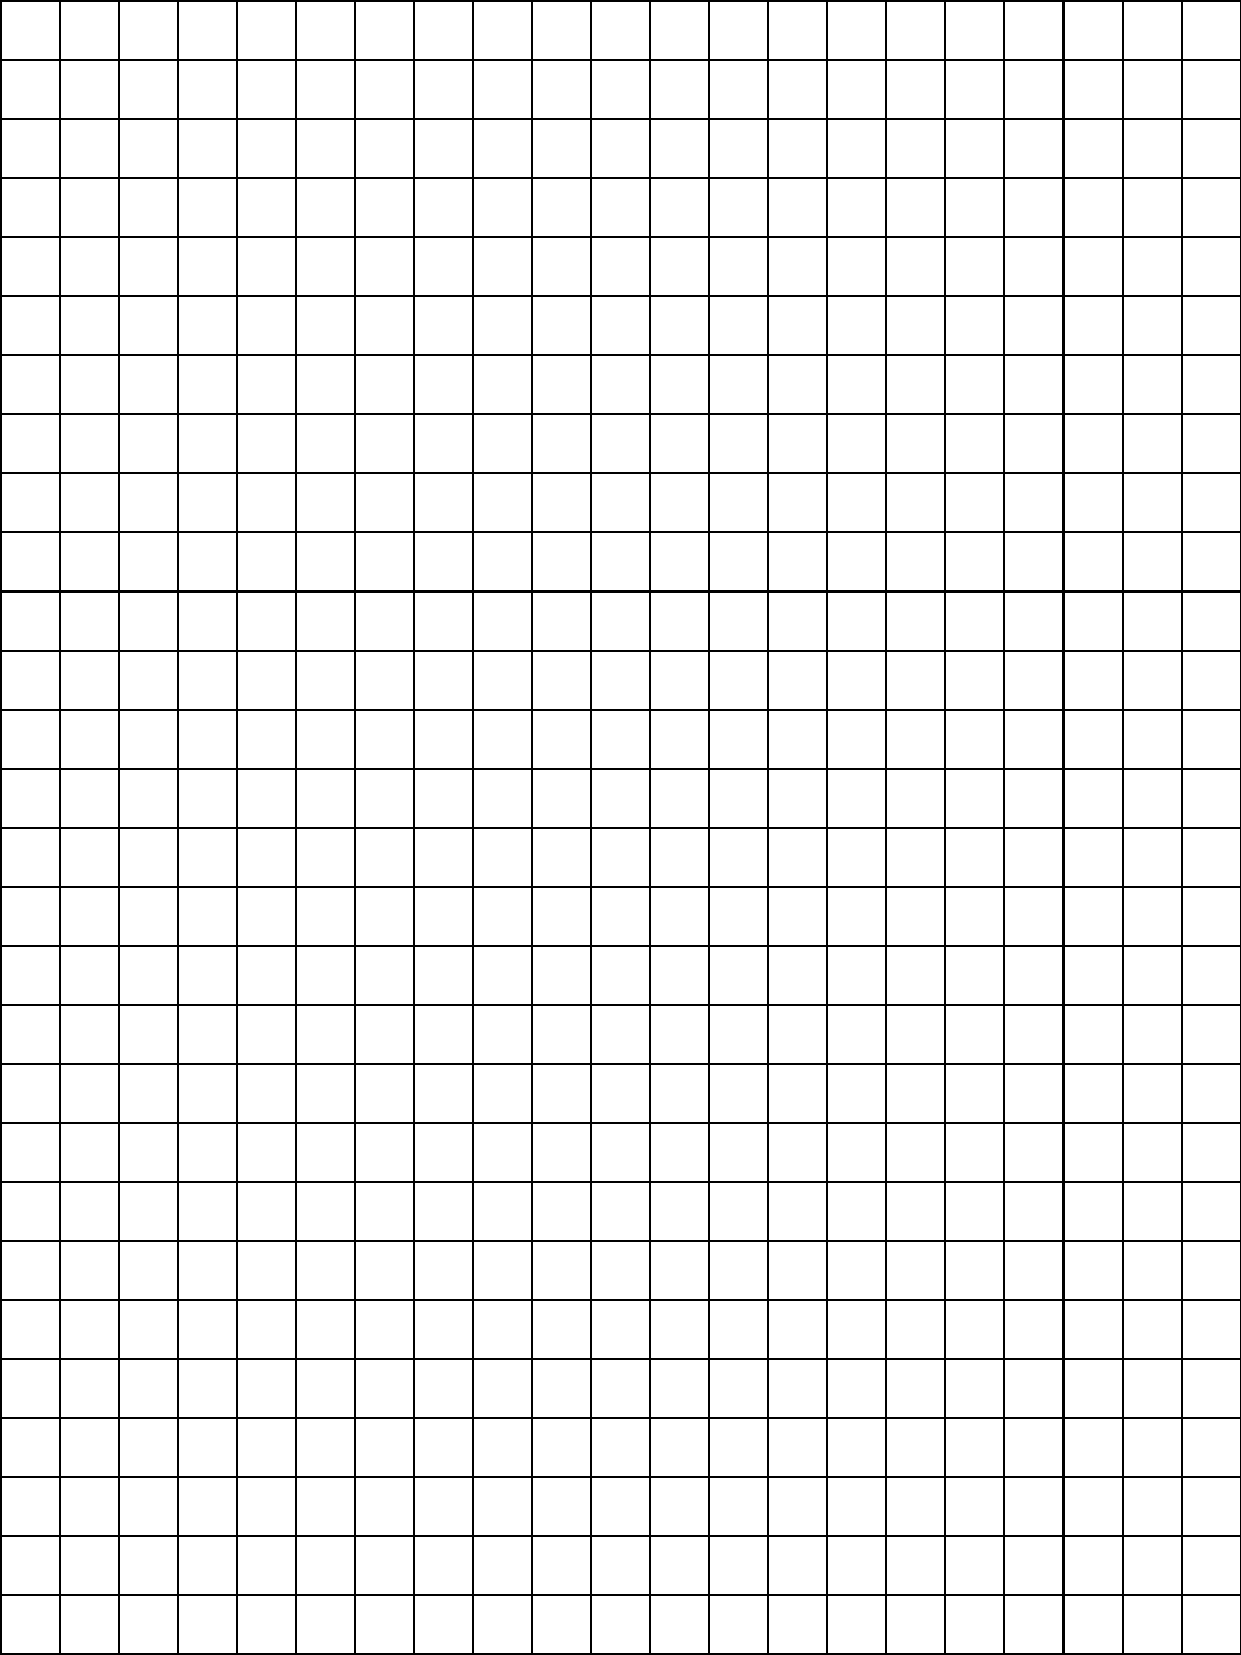
\includegraphics[scale=0.9]{omkr}
\end{center}
\begin{comment}
\newpage
\textbf{Fasit}
\begin{align*}
2x+2y &= x y \\
x &= \frac{y-2y}{x-2} \\
y &= \frac{2x}{x-2}
\end{align*}
Heiltallsløysingar:
\begin{align*}
	x=3\quad,\quad y=6 \\
	x=4\quad,\quad y=4
\end{align*}
\end{comment}
\end{document}